\documentclass[11pt,letterpaper]{article}
\usepackage[T1]{fontenc}
\usepackage[utf8]{inputenc}
\usepackage{lmodern,microtype}
\usepackage[margin=1in]{geometry}
\usepackage{amsmath,amssymb,amsthm,mathtools}
\usepackage{booktabs,longtable,array,enumitem}
\usepackage{tikz}
\usepackage{listings}
\usepackage[hidelinks,breaklinks]{hyperref}
\usepackage{fancyhdr}
\pagestyle{fancy}\fancyhf{}\fancyhead[L]{\small Compressed primitive-power elimination}\fancyhead[R]{\small ProveIt research report}\fancyfoot[C]{\thepage}
\setlength{\headheight}{14pt}
\setlength{\parskip}{4pt}
\setlength{\parindent}{1.2em}
\setlength{\emergencystretch}{2em}
\setcounter{tocdepth}{1}
\newtheorem{theorem}{Theorem}[section]
\newtheorem{lemma}[theorem]{Lemma}
\newtheorem{proposition}[theorem]{Proposition}
\newtheorem{corollary}[theorem]{Corollary}
\theoremstyle{definition}
\newtheorem{definition}[theorem]{Definition}
\newtheorem{example}[theorem]{Example}
\newtheorem{remark}[theorem]{Remark}
\newcommand{\Z}{\mathbb Z}
\newcommand{\N}{\mathbb N}
\newcommand{\F}{F}
\newcommand{\nc}[1]{\langle\!\langle #1\rangle\!\rangle}
\newcommand{\cyc}{\operatorname{cycred}}
\newcommand{\red}{\operatorname{red}}
\newcommand{\ab}{\operatorname{ab}}
\newcommand{\supp}{\operatorname{supp}}
\newcommand{\width}{\operatorname{width}}
\newcommand{\bits}{\operatorname{bits}}
\newcommand{\poly}{\operatorname{poly}}
\newcommand{\SLP}{\mathsf{SLP}}
\newcommand{\PP}{\mathsf{PrimitivePower}}
\newcommand{\UNK}{\texttt{UNKNOT}}
\newcommand{\INC}{\texttt{INCONCLUSIVE}}
\lstset{basicstyle=\small\ttfamily,columns=fullflexible,keepspaces=true,breaklines=true,frame=single,showstringspaces=false}
\title{\textbf{Compressed Christoffel Width and\newline Torsion-Free Primitive-Power Elimination}\\[5pt]
\large Exact rank-two terminals, parallel contraction bounds,\newline and a costed route toward quasi-polynomial unknot recognition}
\author{Research report prepared for the ProveIt project\\
\small Mathematical development and reference implementation prepared with ChatGPT}
\date{8 October 2026}
\begin{document}
\maketitle
\begin{abstract}
We develop a compressed algebraic kernel for the group-certificate branch of
unknot recognition. A cyclically reduced word in a rank-two free group is a
power of a primitive element precisely when it is sign-coherent and its
primitive-slope prefix heights have the minimum possible oscillation. A binary
straight-line program can evaluate this oscillation by two bottom-up passes:
no word expansion, Whitehead descent, compressed string equality, or root
extraction is required. With $S$ grammar nodes and $B$ bits for the maximum
expanded length, the query and certificate replay take
$O(S(B+\log(S+2))+B^2)$ bit operations under standard arithmetic bounds.

For a certified classical knot-group presentation, a primitive-power relation
permits killing its primitive root by torsion-freeness. In rank two this is an
unknot certificate, even when additional relators remain and the generators
are not meridians. In higher rank, a two-generator-supported relation permits
an explicit projection $a\mapsto t^v$, $b\mapsto t^{-u}$. Disjoint projections
can be batched. If unselected relators are kept as raw substitution circuits,
a $d$-round contraction schedule has grammar size at most
$S_0+O(r_0B_0 2^d)$ and can be discovered greedily or checked along a supplied
schedule in $\poly(S_0,r_0,m,B_0)2^{O(d)}$ time. The schedule must actually
succeed; no universal depth or producer bound is asserted.

We also give a complete compressed terminal for certified rank-two one-relator
presentations, a normal-consequence search bound, and an integration plan.
The accompanying implementation passes exhaustive comparison with literal
Whitehead reduction on 29,540 cyclically reduced words, independent replay,
small closed-braid/Jones cross-checks, and large nonuniform compressed tests.
The contribution is the explicit arithmetic kernel and its costed composition
with knot-group certificates, not a claim of first proving rank-two compressed
primitivity or of completing unrestricted quasi-polynomial recognition.
\end{abstract}
\vspace{3pt}
\noindent\textbf{Status.} The local theorems below are proved with their stated
hypotheses. The global quasi-polynomial implication is conditional on a
controlled producer or a successful bounded-depth contraction run. The code
is a tested research package, not an installed modification of the maintained
recognizer and not a Lean formalization.
\clearpage
\tableofcontents
\clearpage

\section{Research objective and relation to the current repository}
\label{sec:scope}
The intended input to the eventual recognizer is a classical knot diagram,
not an arbitrary finite presentation with an unverified label saying that it
is a knot group. The central objective remains a uniform bound of the form
\[
 T(n)\leq \exp\bigl(O((\log(n+2))^c)\bigr)
\]
in the diagram size $n$, for a fixed constant $c$. A fast algebraic subroutine
only contributes to this objective when the cost of reaching its input, the
size of that input, and the correctness of its connection to the original
knot are all included.

The inspected repository has a certificate-oriented architecture. Its
\texttt{group\_certificates.tex} describes reconstruction of the complete
Wirtinger presentation, exact defining-generator eliminations, and Whitehead
moves. Its \texttt{relator\_powers.tex} develops quotient-sized donor deletions
and a pure-letter-power Euclidean kernel. The recent intake synthesis treats
a polynomial compressed terminal for two \emph{certified meridian} generators.
The maintained \texttt{compressed\_search.py} returns an internal search
success only to a wrapper that rebuilds and checks the trace. These are useful
constraints, rather than details to bypass \cite{RepoGroup,RepoPowers,RepoIntake,RepoSearch}.

The present contribution is different in three respects. First, the
rank-two test is a constant-dimensional arithmetic summary of a cyclically
reduced grammar. Second, primitive \emph{powers}, rather than just primitive
relators or pure letter powers, supply an elimination rule in a torsion-free
group. Third, a normalization-free parallel composition gives an explicit
round-depth parameter that controls grammar growth. The terminal does not
require a meridian marking on the current free generators. It does still
require the stronger, indispensable fact that the \emph{whole current
presentation} is the group of the original knot.

\subsection{What is classical, and what is being added}
The classification of primitive conjugacy classes in $F_2$ by coprime lattice
vectors and Christoffel words is classical. We use the formulation in
Kassel--Reutenauer, Theorem~3.2 and Corollary~3.3 \cite{KR}; the earlier work of
Osborne--Zieschang is another standard source \cite{OZ}. Prefix ranges of a
weighted word also form a familiar concatenation monoid. Neither of these
facts is claimed as a new foundational discovery.

Kapovich's July 2026 preprint proves deterministic polynomial-time compressed
primitivity in rank two and describes a Euclidean automorphism construction
followed by one compressed cyclic-reduction test \cite[Section~8]{Kapovich}.
Consequently, ``compressed rank-two primitivity is in $\mathsf P$'' is not a
new complexity-class claim here. Our kernel instead exploits the useful
\emph{already cyclically reduced} interface: after counts and one gcd, it
uses only prefix extrema. It also recognizes all powers of primitive words
and feeds a projection rule for entire presentations. This removes a final
general-purpose reduction from this particular entry interface; it does not
prove a uniformly better bound when arbitrary normalization is included.

The round-depth bound, the distinction between raw circuits and repeated
normalization, and the independent certificate implementation are the main
project-facing results. Priority beyond the sources examined has not been
established. They should be integrated as proved deductions with explicit
hypotheses, not advertised as a resolution of the full recognition problem.

\subsection{Current complexity claims are not interchangeable}
Lackenby's July 2026 manuscript gives an unknot-recognition algorithm through
incompressible surfaces and hierarchies. Section~9 explicitly separates the
number of visits to stages from running-time estimates, because some stages
are not specified sufficiently precisely for the latter \cite[Section~9]{Lackenby}.
This report neither replaces that geometric program nor interprets an
algorithmic announcement as a bound for the repository implementation.
Likewise, a positive certificate kernel, a complete restricted terminal, and
a complete recognizer have different interfaces and are labeled separately
below.

\section{Input model and algebraic conventions}
\label{sec:model}
Let $F_r=F(x_1,\ldots,x_r)$ be the free group on a fixed current basis.
A word is freely reduced if no adjacent letters are mutual inverses. A
nonempty freely reduced word is cyclically reduced if its first and last
letters are not inverses. We include the empty word as cyclically reduced,
but never as a nonzero power of a primitive element. An element is primitive
if it belongs to a free basis. A \emph{primitive-power word} represents
$g u^d g^{-1}$, where $u$ is primitive and $d$ is a nonzero integer. Its inverse
can absorb the sign of $d$, so certificates below use $d>0$.

A binary $\SLP$ is a topologically ordered directed acyclic grammar. Node zero
is empty; each later node is either a signed letter or a concatenation of two
earlier nodes. Multiple root nodes may share subgrammars. Write $S$ for the
number of supplied nodes, including the empty node; $m$ for the number of
relator roots; $L$ for the maximum expanded length of a supplied node, with
$L\geq1$ by convention; and
\[
 B=\max\{1,\lceil\log_2(L+1)\rceil\}.
\]
This maximum is important. If unreachable nodes are supplied and validated,
their lengths are charged as well. Alternatively, prune to the ancestors of
the roots first, retaining the cost of reading and remapping the input.
For binary grammars $B=O(S)$, but $L$ may be exponential in $S$.

The encoded input also contains node identifiers of $O(\log(S+2))$ bits.
We count additions and comparisons of $B$-bit integers in $O(B)$ time.
Classical gcd, exact division, and multiplication may conservatively be
charged $O(B^2)$ each. The classical quadratic bound for an entire Euclidean
gcd computation is used, not the product of a pessimistic quadratic division
bound with a linear number of divisions. All subsequent statements remain
valid with any other fixed polynomial arithmetic bounds.

For $F(a,b)$ write
\[
 \ab(W)=(\sigma_a(W),\sigma_b(W)).
\]
A word is \emph{sign-coherent} when neither generator appears with both signs.
After independently inverting $a$ and $b$, every nonempty sign-coherent word
is positive. Counts of absent generators are zero; their sign choice is
irrelevant. All word-level negative answers assume that the root is actually
cyclically reduced. Invalid normalization is a precondition failure, not a
non-primitivity answer.

\section{Minimum Christoffel width}
\label{sec:width}
We first prove the arithmetic test, including its power version. Let $W$ be a
positive word with $P$ letters $a$ and $Q$ letters $b$, not both zero. Put
\[
 d=\gcd(P,Q),\qquad p=P/d,\quad q=Q/d,\quad \ell=p+q.
\]
For the prefix of length $j$, let $A_j,B_j$ count its $a$ and $b$ letters and
set
\begin{equation}
 H_j=qA_j-pB_j,\qquad
 \Omega(W)=\max_{0\leq j\leq P+Q}H_j-
            \min_{0\leq j\leq P+Q}H_j.
 \label{eq:height}
\end{equation}
The empty prefix and the full prefix are included. In particular,
$H_0=H_{P+Q}=0$.

\begin{lemma}[The unavoidable width]
\label{lem:lowerwidth}
If $p,q>0$, then $\Omega(W)\geq p+q-1$.
\end{lemma}
\begin{proof}
Every $a$ step adds $q$ and every $b$ step adds $-p$. Modulo $\ell=p+q$ these
increments are equal. Thus $H_j\equiv jq\pmod\ell$. Coprimality of $p,q$
implies $\gcd(q,\ell)=1$, so the first $\ell$ prefix heights represent all
$\ell$ residues. An interval of integer width less than $\ell-1$ contains
fewer than $\ell$ integers. It cannot contain these heights.
\end{proof}

\begin{lemma}[Equality forces a periodic rotation path]
\label{lem:rotation}
Suppose $p,q>0$ and $\Omega(W)=\ell-1$. Then $W$ is a repetition, $d$ times,
of a cyclic conjugate of a Christoffel word with counts $(p,q)$.
\end{lemma}
\begin{proof}
Let $h=\min H_j$. Every height lies in
$I=\{h,h+1,\ldots,h+\ell-1\}$. The possible next heights from an integer
$z\in I$ are $z+q$ and $z-p$, which differ by exactly $\ell$.
Exactly one is in $I$: the first is in $I$ precisely when
$z\leq h+p-1$, and the second precisely when $z\geq h+p$.
Therefore the next letter is determined by the current height. This is the
rotation $z-h\mapsto z-h+q\pmod\ell$, realized on consecutive integer
representatives. It visits all heights and returns after exactly $\ell$
steps. Its letters consist of $p$ occurrences of $a$ and $q$ of $b$.
Starting at a different point merely cyclically rotates the same word.
Since $|W|=d\ell$, $W$ follows this cycle exactly $d$ times. The rotation
word is the usual lower Christoffel word, up to the conventional choice of
initial point.
\end{proof}

\begin{lemma}[Christoffel roots are primitive]
\label{lem:primitiveC}
For coprime $p,q\geq0$, the rotation word $C(p,q)$ starting at height zero
is primitive in $F(a,b)$.
\end{lemma}
\begin{proof}
The boundary cases are $C(1,0)=a$ and $C(0,1)=b$. For $p\geq q>0$ write
$p=kq+r$. The rotation path decomposes into $b$ steps preceded by $k$ or
$k+1$ occurrences of $a$, and gives
\begin{equation}
 C(p,q)=\phi_k(C(r,q)),\qquad
 \phi_k(a)=a,\quad \phi_k(b)=a^k b.
 \label{eq:euclid1}
\end{equation}
One can verify the block description directly from the rule in
Lemma~\ref{lem:rotation}: before a $b$ step the height must reach at least
$p$, and removing $k$ $a$ steps per $b$ leaves the rule for $(r,q)$.
Similarly, when $q=kp+r>p$,
\begin{equation}
 C(p,q)=\psi_k(C(p,r)),\qquad
 \psi_k(a)=ab^k,\quad \psi_k(b)=b.
 \label{eq:euclid2}
\end{equation}
Both maps are Nielsen automorphisms, with the indicated powers negated in
their inverses. Euclidean descent reaches one of the boundary cases, so
$C(p,q)$ is an automorphic image of a generator. These are also the standard
Christoffel morphisms; compare \cite[Section~3]{KR}.
\end{proof}

\begin{theorem}[Exact primitive-power width criterion]
\label{thm:width}
Let $W$ be a nonempty cyclically reduced word in $F(a,b)$. The following are
equivalent:
\begin{enumerate}[label=(\roman*),nosep]
\item $W$ is a conjugate of a nonzero power of a primitive element;
\item $W$ is sign-coherent and, after its sign normalization,
\[
 \Omega(W)=p+q-1.
\]
\end{enumerate}
When these conditions hold, the primitive-power exponent is
$d=\gcd(P,Q)$. In particular, $W$ itself is primitive exactly when $d=1$.
The criterion includes pure one-letter words, where $\ell=1$ and the width
is zero.
\end{theorem}
\begin{proof}
For a positive word with both letters, equality implies the assertion by
Lemmas~\ref{lem:rotation} and \ref{lem:primitiveC}. The cyclic root has counts
$(p,q)$, so it cannot be a further proper power: any such power would divide
both $p$ and $q$. This proves the exponent assertion.

For the converse, cyclically reduce a primitive root. The classical
rank-two classification says that this root is a cyclic conjugate of a
Christoffel word after independently choosing the signs of the generators
\cite[Corollary~3.3]{KR}. Since the root is cyclically reduced, its positive
powers have no cancellations at their joins. A cyclically reduced conjugate
is a cyclic rotation. It is therefore sign-coherent and traverses the same
$\ell$-height rotation cycle repeatedly, with width $\ell-1$.
For a single occurring generator the reduced word is a nonzero power of that
generator, and the stated zero-width computation is immediate. Finally,
a proper power cannot be primitive because its abelianization vector is
not primitive.
\end{proof}

\subsection{Signed implementation formula}
Instead of changing the grammar, compute the signed exponent vector
$(U,V)$ and $d=\gcd(|U|,|V|)$. For a nonempty coherent root $d>0$. Put
$(u,v)=(U/d,V/d)$ and give the original signed letters the weights
\begin{equation}
 a\mapsto v,\quad a^{-1}\mapsto-v,\quad
 b\mapsto-u,\quad b^{-1}\mapsto u.
 \label{eq:signedweights}
\end{equation}
These heights are either the normalized heights or their negatives, so
oscillation is unchanged. The acceptance threshold is $|u|+|v|-1$.
This avoids changing leaf labels and deals uniformly with negative slopes.

\subsection{A necessary safeguard against abelianization shortcuts}
For coprime $p,q>1$, the positive block word $a^p b^q$ has height range
$[0,pq]$. Its excess over the minimum is exactly
\begin{equation}
 \Omega(a^p b^q)-(p+q-1)=(p-1)(q-1)>0.
 \label{eq:blockdefect}
\end{equation}
Thus coprime exponent sums emphatically do not imply primitivity.
The presentation $\langle a,b\mid a^2b^{-3}\rangle$, for example, is the
standard trefoil presentation, and its normalized word has width $6$ rather
than the required $4$. The arithmetic test distinguishes order information
that the exponent vector loses.

\begin{figure}[ht]
\centering
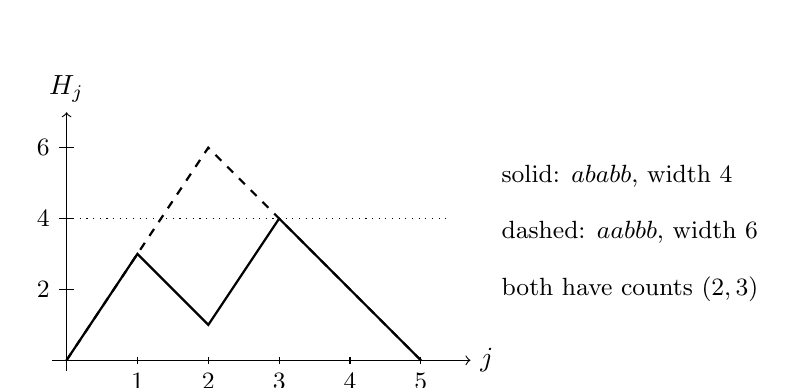
\begin{tikzpicture}[x=0.9cm,y=0.45cm]
\draw[->](-0.2,0)--(5.7,0) node[right]{$j$};
\draw[->](0,-0.3)--(0,7) node[above]{$H_j$};
\foreach \x in {1,...,5} {\draw(\x,0.1)--(\x,-0.1) node[below] {\small\x};}
\foreach \y in {2,4,6} {\draw(0.1,\y)--(-0.1,\y) node[left]{\small\y};}
\draw[dotted] (0,4)--(5.4,4);
\draw[thick] (0,0)--(1,3)--(2,1)--(3,4)--(4,2)--(5,0);
\draw[thick,dashed] (0,0)--(1,3)--(2,6)--(3,4)--(4,2)--(5,0);
\node[anchor=west] at (6,5.2) {\small solid: $ababb$, width $4$};
\node[anchor=west] at (6,3.6) {\small dashed: $aabbb$, width $6$};
\node[anchor=west] at (6,2) {\small both have counts $(2,3)$};
\end{tikzpicture}
\caption{Minimum-width Christoffel order versus the same coprime counts in
nonprimitive block order. The comparison is exact over the integers.}
\label{fig:width}
\end{figure}

\section{Two-pass compressed queries and independent replay}
\label{sec:algorithm}
For each grammar node store its four signed occurrence counts, its first and
last letters, its length, and a freely reduced flag. At a concatenation $XY$,
counts and lengths add. Endpoints are inherited from the nonempty children.
The reduced flag is true exactly when both child flags are true and either a
child is empty or the last letter of $X$ is not the inverse of the first letter
of $Y$. A root is cyclically reduced exactly when this flag is true and its
nonempty endpoints are not inverses. Induction on the grammar proves all
these statements without expansion.

Once the slope is fixed, define the profile of a word by
\[
 \mathcal P(X)=(t_X,m_X,M_X),
\]
where $t_X$ is its total weight and $m_X,M_X$ are its minimum and maximum
prefix weights, including the empty prefix. A letter of weight $w$ has
profile $(w,\min(0,w),\max(0,w))$. The empty word has profile $(0,0,0)$.

\begin{lemma}[Prefix-profile product]
\label{lem:monoid}
For any two words, with no reduction performed,
\begin{equation}
 (t,m,M)\star(s,n,N)
 =\bigl(t+s,\min(m,t+n),\max(M,t+N)\bigr)
 \label{eq:monoid}
\end{equation}
is the profile of their concatenation. This product is associative.
\end{lemma}
\begin{proof}
Every prefix of $XY$ is either a prefix of $X$ or all of $X$ followed by a
prefix of $Y$. Their weights form the union of the prefix-weight set of $X$
and its translate by $t_X$ of the prefix-weight set of $Y$. This proves the
formula. Applying the same description to three successive prefix sets
proves associativity, or it follows from associativity of concatenation and
the explicit formulas for extrema.
\end{proof}

\begin{theorem}[Compressed query bound]
\label{thm:query}
On a validated binary $\SLP$ with cyclically reduced root, primitive-power
recognition and extraction of $(u,v,d,\Omega)$ take
\begin{equation}
 O\bigl(S(B+\log(S+2))+B^2\bigr)
 \label{eq:localcost}
\end{equation}
bit operations and $O(SB+S\log(S+2))$ bits of working storage.
A certificate consisting of the root identifier and these four integers can
be independently checked within the same asymptotic bound. The bound becomes
$O(S^2)$ for binary grammars, up to harmless small-input conventions.
\end{theorem}
\begin{proof}
The count/endpoint pass has constant-dimensional integer summaries. Counts
are at most $L$. The gcd and exact divisions have the stated quadratic bit
cost. Each letter weight has $O(B)$ bits and every prefix height has absolute
value at most $L^2$, hence at most $2B+O(1)$ bits. Formula~\eqref{eq:monoid}
uses only a fixed number of additions and comparisons per node. Reading
and validating pointers contributes $O(S\log(S+2))$.

For replay, derive all counts and endpoints afresh from the original grammar,
check $d>0$, $\gcd(|u|,|v|)=1$, $\ab(W)=d(u,v)$, sign coherence and cyclic
reduction, and recompute the profile using weights~\eqref{eq:signedweights}.
Finally check $\Omega=|u|+|v|-1$. The verifier need not trust any producer
summary. Storing total weights per node avoids multiplying a slope by a
count vector at every internal node; only a constant number of final integer
products are needed. The same bound follows. Since $B=O(S)$, both passes are
quadratic in the binary grammar-node parameter in the worst case.
\end{proof}

\subsection{What is deliberately not inside this bound}
The root must already be cyclically reduced. General compressed free and
cyclic reduction are polynomial-time operations, by Lohrey's results as
exposed in Schleimer \cite[Theorem~3.3 and Corollary~3.6]{Schleimer}.
If normalization maps an input of size $S$ to an output of size $S'$, the
correct combined bound is
\[
 T_{\rm normalization}(S)+O\bigl(S'(B'+\log(S'+2))+(B')^2\bigr),
\]
not automatically the right side of~\eqref{eq:localcost} with the old $S$.
The standalone reference kernel rejects an unreduced input; it does not
pretend to implement this general normalization theorem. The inspected
repository already has a separate exact compressed-word backend
\cite{RepoWords}.

The code uses no random fingerprints, approximate equality, floating-point
heights, or expanded-length loops in the kernel. Its resource limits are
interrupts. Exceeding a node, bit-length, or external cancellation budget
cannot return a mathematical negative answer.

\section{Shared scans over all relators}
\label{sec:shared}
For a genuine two-generator knot-group presentation, the integer exponent
matrix has row lattice of rank one: its cokernel is the knot abelianization
$\Z$. Thus all nonzero exponent rows lie on one rational line. From one
nonzero row compute a primitive direction $(u,v)$, choosing its sign
canonically. Collinearity of another row $(A,B)$ is exactly
\[
 vA-uB=0.
\]
A single profile pass with weights $(v,-u)$ then supplies the widths of
\emph{all} relator roots in the shared grammar.

\begin{proposition}[Shared-slope scan]
\label{prop:shared}
For $m$ cyclically reduced roots with collinear exponent vectors, one profile
pass identifies every primitive-power root. A conservative bit bound is
\begin{equation}
 O\bigl(S(B+\log(S+2))+m(B^2+\log(S+2))\bigr).
 \label{eq:sharedcost}
\end{equation}
\end{proposition}
\begin{proof}
Use the common direction for the profile pass. For each nonempty coherent
root with exponent vector $(A,B)\ne(0,0)$, let
$d=\gcd(|A|,|B|)$. Its own primitive direction is either $(u,v)$ or its
negative. Negating weights leaves width unchanged, so the common threshold
$|u|+|v|-1$ applies. A nonempty root with zero exponent vector cannot be a
primitive power. Theorem~\ref{thm:width} therefore decides every root.
Collinearity tests, per-root gcds, and exact arithmetic can be charged
$O(mB^2)$; they must not be described as unit-cost merely because the
profile itself uses only additions.
\end{proof}

This is a reuse optimization, not an inference of topology from Smith normal
form. Collinearity alone does not even show that the abelianization is
$\Z$: the gcd of the scalar row multiples must also be one. More importantly,
abelianization $\Z$ does not show that a presentation is a classical knot
group. A verified geometric origin and an equivalence trace are still needed
before invoking torsion-freeness or the unknot theorem.

\section{From primitive powers to whole-presentation elimination}
\label{sec:groups}
The following topological facts form a small, explicit interface to the
algebra. A classical knot exterior is irreducible, its first homology is
$\Z$, and its fundamental group is torsion-free. For torsion-freeness, one
may use asphericity together with the fact that a group admitting a
finite-dimensional classifying space has no nontrivial finite cyclic
subgroup; see \cite[(C.1)--(C.2)]{AFW}. The classical Dehn/Loop Theorem implies
that a knot group is infinite cyclic precisely for the unknot
\cite{Papakyriakopoulos}.

For completeness, the latter implication can be seen directly at the
boundary torus. If $\pi_1(E_K)=\Z$, the inclusion-induced map
$\pi_1(\partial E_K)=\Z^2\to\pi_1(E_K)$ cannot be injective. The Loop Theorem
gives a compressing disk. An irreducible orientable knot exterior with
compressible torus boundary is a solid torus: compressing the boundary gives
a sphere, which bounds a ball, and reversing the compression attaches a
single one-handle. The knot is therefore the unknot. These facts apply to
classical knots in $S^3$, not to arbitrary links, virtual diagrams, or
presentations with only a matching abelianization.

\begin{theorem}[Torsion-free root elimination]
\label{thm:rootkill}
Suppose a presentation $\langle X\mid\mathcal R\rangle$ presents a torsion-free
group $G$. If an actual relator or a verified normal consequence is a conjugate
of $w^d$, with $d\ne0$ and $w$ primitive in $F(X)$, then adding $w=1$ preserves
$G$. In a basis containing $w$, one may eliminate its generator and project
\emph{all} remaining relators.
\end{theorem}
\begin{proof}
The represented element satisfies $w^d=1$ in $G$. Torsion-freeness implies
$w=1$ already in $G$, so adjoining that relation makes no further quotient.
Primitivity supplies a basis with first member $w$. The added relation kills
that generator, and the usual defining-generator elimination gives the
claimed presentation on one fewer generator. All other relators are
substituted rather than discarded.
\end{proof}

\begin{remark}[A root rule is not an unrestricted Tietze rule]
The presentation $\langle a,b\mid a^2\rangle$ defines $C_2*\Z$.
Replacing $a^2$ by $a$ changes it to $\Z$. Thus a syntactic primitive-power
certificate is not by itself a proof that root extraction preserves an
arbitrary presented group. When $d=1$, the extra torsion-free hypothesis is
unnecessary; for $d>1$ it must be justified by the caller's verified context.
\end{remark}

\subsection{An explicit two-letter projection without basis expansion}
\begin{theorem}[Fused primitive-pair projection]
\label{thm:projection}
Let $w$ be primitive in the free factor $F(a,b)\leq F(X)$, with
$\ab(w)=(u,v)$ and $\gcd(|u|,|v|)=1$. Let $t$ be a new generator and define
\begin{equation}
 \pi(a)=t^v,\qquad \pi(b)=t^{-u},\qquad
 \pi(x)=x\quad(x\in X\setminus\{a,b\}).
 \label{eq:projection}
\end{equation}
Then
\[
 F(X)/\nc{w}\cong F\bigl((X\setminus\{a,b\})\cup\{t\}\bigr)
\]
via $\pi$. Consequently, under Theorem~\ref{thm:rootkill}, a two-letter
primitive-power relation permits replacing every relator by its image under
\eqref{eq:projection}. There is no need to expand a Nielsen basis or a
conjugating word.
\end{theorem}
\begin{proof}
Because $w$ is primitive, $F(a,b)/\nc{w}$ is infinite cyclic. The character
$a\mapsto v$, $b\mapsto-u$ annihilates $w$ and is surjective because
$\gcd(|u|,|v|)=1$. Hence the induced epimorphism from this infinite cyclic
quotient to $\Z$ is an isomorphism, and its kernel in $F(a,b)$ is exactly
$\nc{w}$. Passing to the free product with the remaining generators proves
the assertion. More explicitly, Bezout coefficients $\alpha,\beta$ satisfying
$v\alpha-u\beta=1$ give the inverse generator $t=\overline{a^\alpha b^\beta}$
in the quotient. No commutativity is imposed on the other free generators.
\end{proof}

The root detected by Theorem~\ref{thm:width} is only specified up to conjugacy
and inversion. Neither ambiguity changes its normal closure. A primitive
of a free factor $F(a,b)$ remains primitive in $F(X)$ by extending its basis
with the other generators. These observations discharge both potential
ambiguities in using the local classifier inside a larger presentation.

\begin{corollary}[Two arbitrary generators suffice at the positive terminal]
\label{cor:unknot}
Let $\langle a,b\mid R_1,\ldots,R_m\rangle$ be certified to present the group
of a classical knot. If any actual relator or verified normal consequence is
a nonzero power of a primitive element of $F(a,b)$, then the knot is the
unknot.
\end{corollary}
\begin{proof}
Root elimination makes the presented group a quotient of an infinite cyclic
group. Since its abelianization is $\Z$, this quotient is $\Z$ itself.
The knot-group criterion above finishes the proof. No remaining relation
needs to be assumed redundant, and neither $a$ nor $b$ needs to be a meridian.
\end{proof}

Failure to find such a relation in a supplied multi-relator list is only a
failure of that positive terminal. It is not a nontrivial-knot certificate.
An unknown relation in the normal closure may still have the required form.

\subsection{An exact family without any torsion-free hypothesis}
\begin{theorem}[Aligned primitive-power presentations]
\label{thm:aligned}
Suppose every nonempty relator of a rank-two presentation is a primitive
power and all their primitive exponent vectors lie on the same line. Let
$d_1,\ldots,d_s>0$ be their exponents and $g=\gcd(d_1,\ldots,d_s)$.
Then the presented group is $C_g*\Z$, with $C_1$ trivial. If all relators
are empty, the group is $F_2$ instead.
\end{theorem}
\begin{proof}
Primitive vectors on a fixed integral line differ only by sign. By the
rank-two classification, the primitive roots are conjugate to a fixed
primitive word $w$ or to $w^{-1}$ \cite{KR}. Thus their normal closure is
$\nc{w^{d_1},\ldots,w^{d_s}}$. Bezout's identity shows that $w^g$ is a product
of integer powers of these elements, and every $w^{d_i}$ is a power of $w^g$.
The normal closure is exactly $\nc{w^g}$. Completing $w$ to a basis produces
$\langle w,z\mid w^g\rangle=C_g*\Z$.
\end{proof}

For instance, take a nonuniform Christoffel word $C$ and compressed exponents
$N=2^h$, $N^2+1$. The two-relator presentation
\[
 \langle a,b\mid C^N,C^{N^2+1}\rangle
\]
is infinite cyclic. The shared width/gcd scan proves this without repeatedly
subtracting a donor or comparing differently parsed copies of $C$.
This extends the repository's pure-letter arithmetic example to a
nonuniform primitive root and to independently rotated relators. It does
not show that an arbitrary input knot has such a presentation.

\begin{proposition}[A primitive anchor classifies arbitrary additional relators]
\label{prop:anchor}
If one relator $R$ is primitive with exponent vector $(u,v)$, then
\[
 \langle a,b\mid R,W_1,\ldots,W_k\rangle
 \cong \Z/h\Z,\qquad
 h=\gcd_i\bigl|v\sigma_a(W_i)-u\sigma_b(W_i)\bigr|,
\]
where $h=0$ means $\Z$.
\end{proposition}
\begin{proof}
Quotient by $R$ using Theorem~\ref{thm:projection}. Each remaining relator
becomes a power of $t$ with the displayed exponent. Relations in a cyclic
group generate the subgroup determined by their gcd.
\end{proof}
This is an unconditional algebraic statement. It is useful for independently
checking that no remaining relator was silently forgotten.

\section{A complete rank-two one-relator terminal}
\label{sec:onereletor}
\begin{theorem}[One-relator cyclicity]
\label{thm:onereletor}
For a nonempty word $R\in F(a,b)$,
\[
 \langle a,b\mid R\rangle\cong\Z
 \quad\Longleftrightarrow\quad R\text{ is primitive in }F(a,b).
\]
Hence, on a certified rank-two one-relator knot-group presentation, normalize
$R$ once and apply Theorem~\ref{thm:width}, accepting precisely when the
primitive-power exponent is one. This is a complete decision at that
interface, not merely a positive test.
\end{theorem}
\begin{proof}
The forward implication uses the Magnus normal-closure theorem: two elements
of a free group with the same normal closure are conjugate or
inverse-conjugate \cite{Magnus,Howie}. Let the quotient map to $\Z$ send
$a,b$ to coprime integers $A,B$. A Nielsen change of basis transforms this
primitive character to the coordinate projection $F(s,t)\to\Z$ with
$s\mapsto0$, $t\mapsto1$. Its kernel is $\nc{s}$. Translated back to the
original basis, there is a primitive $w$ such that
$\nc{R}=\ker(F_2\to\Z)=\nc{w}$. Magnus's theorem makes $R$ conjugate to
$w$ or $w^{-1}$, hence primitive. Conversely, quotienting a free basis by
one of its members leaves an infinite cyclic group.
\end{proof}

If $R$ cyclically reduces to the empty word, the presentation is $F_2$ and
not cyclic. In a purported knot presentation this also fails the necessary
abelianization test. The topology wrapper must distinguish invalid input
provenance from a nontrivial-knot outcome.

It is essential not to extend the negative direction to an arbitrary
multi-relator presentation. For example,
$\langle a,b\mid (ab)^2,(ab)^3\rangle\cong\Z$, although neither relator is
primitive. This also illustrates why the torsion-free positive terminal
and the aligned-family theorem are useful alongside the one-relator test.

\subsection{A justified deficiency-one starting presentation for braids}
A closed $r$-strand braid has the Artin presentation
\[
 \langle x_1,\ldots,x_r\mid \beta(x_i)x_i^{-1},\ 1\leq i\leq r\rangle.
\]
Each local Artin automorphism preserves $x_1\cdots x_r$. If the first $r-1$
relations hold, the equality
$\beta(x_1)\cdots\beta(x_r)=x_1\cdots x_r$ implies the last relation.
Thus the last relator can be removed with this explicit justification.
Starting with the resulting $r-1$ relators, each defining-generator
elimination removes one generator and one defining relation. At rank two,
there is one remaining designated relation, possibly accompanied by empty
slots. The endpoint criterion above therefore applies whenever such a
certified reduction reaches it.

The supplied braid demonstration conservatively retains all Artin relators
and implements only the positive terminal. The deficiency-one deletion and
the complete negative endpoint are proved here but are not represented as
already installed production features.

\section{Parallel contractions with an explicit grammar-growth bound}
\label{sec:rounds}
The next result addresses a different bottleneck: composing many safe local
reductions without repeatedly paying an uncontrolled normalization cost.
The crucial restriction is stated as part of the algorithm, not left implicit.

\begin{definition}[Normalization-free contraction round]
At the start of a round the presentation is represented by a shared binary
grammar, whose relators may be unreduced. Select some current relator roots
whose \emph{spelled words} are cyclically reduced primitive powers supported
on pairwise disjoint pairs of current generators. Verify their local
certificates. Apply all maps~\eqref{eq:projection} simultaneously, and retain
all other relators as raw substitution circuits. A selected donor may be
replaced by an empty root after the checked projection, since its image is
freely trivial by Theorem~\ref{thm:projection}. Its old slot and proof record
remain in the trace. No free or cyclic reduction is run on the other roots.
\end{definition}

Disjointness is a syntactic condition on generator support. It makes the
maps independent and allows all new image powers to be built before one
pass through the old grammar. It is not a claim that arbitrary overlapping
primitive roots commute as elimination operations.

\begin{theorem}[Normalization-free round-depth bound]
\label{thm:roundbound}
Let an initial torsion-free presentation have $r_0$ generators, $m$ relator
slots, $S_0$ grammar nodes, and maximum length-bit bound $B_0$. For a run of
$d$ nonempty normalization-free contraction rounds using current relators,
there is an implementation satisfying
\begin{align}
 B_j&\leq 2^jB_0, \label{eq:Bbound}\\
 S_j&\leq S_0+C r_0B_0(2^j-1) \label{eq:Sbound}
\end{align}
for an absolute constant $C$, after pruning or remapping unreachable nodes.
The run can be checked along a supplied schedule, or produced by the explicit
greedy disjoint-pair scan until it stalls, in
\begin{equation}
 \poly(S_0,r_0,m,B_0)\,2^{O(d)}
 \label{eq:roundtime}
\end{equation}
bit operations. Here a ``run of $d$ rounds'' means the rounds that actually
occur; the theorem does not say that the run reaches one or two generators.
\end{theorem}
\begin{proof}
Let $L_j\geq1$ be the maximum expanded node length at round $j$.
For every accepted pair, the primitive coordinates $u,v$ have absolute
values at most the length of its relator, hence at most $L_j$. Each original
letter is therefore replaced by a power of length at most $L_j$, or by a
single unaffected letter. Every old node expands to at most $L_j^2$ letters.
New power nodes have length at most $L_j$. Thus
$L_{j+1}\leq L_j^2$, with the convention $L_j\geq1$, and
$\lceil\log_2(L_j^2+1)\rceil\leq 2B_j$. This proves
\eqref{eq:Bbound} by induction.

Binary powering constructs the positive and negative images for a generator
pair with $O(B_j)$ new nodes. There are at most $r_0/2$ pairs. Copy each
reachable old concatenation at most once, redirecting leaves to their image
roots; shared images and shared old subexpressions are not expanded. This
gives
\[
 S_{j+1}\leq S_j+C r_0B_j.
\]
Summing this recurrence and~\eqref{eq:Bbound} proves~\eqref{eq:Sbound}.
Empty donor slots need no extra nonempty nodes.

To find eligible relators, compute endpoints, reduced flags, and supports.
It is enough to remember at most three distinct support labels: three
already makes a root ineligible for this two-letter kernel. For each
eligible two-letter root, extract and rename its ancestor grammar and apply
Theorem~\ref{thm:query}. Even a separate scan for every relator costs a fixed
polynomial in $S_j,m,r_0,B_j$. A greedy disjoint matching is another polynomial
operation; no enumeration of all matchings is required for this stated run.
Similarly a supplied matching can be checked in polynomial time. Substitution
and node remapping have polynomial bit cost. There are at most $r_0-1$
nonempty rank-reducing rounds. Substituting~\eqref{eq:Bbound}--\eqref{eq:Sbound}
into a fixed polynomial and summing yields~\eqref{eq:roundtime}.

Finally, the group stays unchanged by Theorems~\ref{thm:rootkill} and
\ref{thm:projection}. Each simultaneous set of killed primitive roots is
already trivial in the current torsion-free group. The quotient of the free
group by their normal closure is the free product of the corresponding
rank-one factors and the unaffected generators. Projecting every remaining
relator gives the same presented group. Torsion-freeness is thus available
again in the next round.
\end{proof}

\begin{corollary}[A quantitative restricted route]
\label{cor:quasi}
Suppose an $n$-size knot input is converted, with a verified trace and cost
$V(n)$, to a presentation with $S_0,r_0,m,B_0\leq n^{O(1)}$. If a produced
normalization-free run reaches a valid cyclic terminal in $d$ rounds, its
additional work is $n^{O(1)}2^{O(d)}$. In particular, $d=O(\log n)$ gives
polynomial additional work, and $d=O((\log n)^2)$ gives
$n^{O(\log n)}$ additional work.

A complete restricted recognizer results if the producer is guaranteed to
reach a rank-two one-relator endpoint on every input in the promised class,
with the stated bounds, and its final normalization and empty-relator checks
are performed once by a fixed polynomial compressed-word algorithm.
\end{corollary}
\begin{proof}
Apply Theorem~\ref{thm:roundbound}. At a one-generator endpoint, each raw
relator reduces to a power determined by its exponent sum, so cyclicity can
be checked without expanded reduction. At a rank-two one-relator endpoint,
use Theorem~\ref{thm:onereletor}. A fixed polynomial final normalization on a
grammar of size $n^{O(1)}2^{O(d)}$ stays within that form. The cost $V(n)$ is
added, not suppressed.
\end{proof}

\subsection{Why not normalize every round?}
Suppose all that is known about a normalization routine is that it maps a
grammar of size $S$ to one of size at most $S^c$. Calling it after every round
permits a recurrence $S_{j+1}\leq(S_j+C r_0B_j)^c$. Iteration can produce a
bound with an exponent depending exponentially on $j$. Merely calling each
individual step ``polynomial'' does not give~\eqref{eq:roundtime}.
The raw-circuit restriction avoids this issue. It may make the search stall
sooner because an algebraically useful but unreduced relator is ineligible.
That loss of applicability is explicit and is the subject of a research
question, not something concealed by a free normalization oracle.

\subsection{What the depth parameter does not prove}
A small maximal matching in one round need not lead to a favorable later
presentation. Even if some sequence of choices reaches a good endpoint,
a particular greedy schedule might not. The theorem bounds the work of a
specified successful run, or of the particular greedy run that is actually
produced; it does not turn an existential good schedule into a polynomial
search for one. A search over schedules must have its own branching bound.

Likewise, the theorem uses \emph{current relators}. Replacing that requirement
by ``some short-looking normal consequence exists'' introduces a proof-search
cost. The next section records one honest way to charge that cost.

\section{A canonical normal-consequence target and its search cost}
\label{sec:consequences}
The preceding terminal accepts a suitable relation once it is present. There
is also a useful way to specify exactly what an unrestricted positive search
would need to prove at a certified rank-two interface.

\begin{theorem}[A fixed primitive target]
\label{thm:target}
Suppose $P=\langle a,b\mid R_1,\ldots,R_m\rangle$ has abelianization $\Z$.
Let the lattice generated by the exponent vectors of the relators be
$\Z(u,v)$, with $\gcd(|u|,|v|)=1$. Choose the signed Christoffel word $C$
with exponent vector $(u,v)$. Then
\[
 P\cong\Z\quad\Longleftrightarrow\quad
 C\in\nc{R_1,\ldots,R_m}\subset F(a,b).
\]
In particular, for a certified classical knot-group presentation, this
normal-closure membership condition is equivalent to unknottedness.
\end{theorem}
\begin{proof}
Every relator has zero image under the primitive character
$\chi(a)=v$, $\chi(b)=-u$. The kernel of this character is $\nc{C}$, by
Theorem~\ref{thm:projection}. Thus $N=\nc{R_1,\ldots,R_m}\subseteq\nc{C}$.
If $C\in N$, equality holds and the quotient is $\Z$. Conversely, if
$F_2/N\cong\Z$, the map induced by $\chi$ is an epimorphism from $\Z$ to
$\Z$, hence an isomorphism. Its kernel is zero, so $N=\ker\chi=\nc{C}$.
The final assertion uses the knot-group criterion.
\end{proof}

The lattice hypothesis is more than pairwise collinearity: the greatest
common divisor of the integer multiples on the primitive line must be one.
It is supplied automatically by a correct knot-group provenance chain, or
can be checked arithmetically as a necessary consistency condition. It is
not itself a proof that the presentation comes from a knot.

The Euclidean construction of Lemma~\ref{lem:primitiveC} builds $C$ as a
small grammar. A conservative $O(B^2)$ node bound follows from $O(B)$
Euclidean stages, each using binary powers of $B$-bit quotients; a more
careful sum of quotient bit lengths gives $O(B)$ nodes. Either bound is
polynomial. A small target is therefore available without solving the
membership problem. This distinction prevents an important circular
argument: the exponent vector identifies the target, but it does not prove
that the target is a consequence of the original relations.

\begin{definition}[Normal-derivation program]
A program starts with the $m$ input relators, regarded as identities in the
presented group. A new instruction may invert an earlier identity, multiply
two earlier identities, or conjugate an earlier identity by one signed
basis letter. The program length is the number of new instructions. A
chosen output is a \emph{verified normal consequence} after its instruction
list has been replayed.
\end{definition}

\begin{proposition}[A costed bounded search]
\label{prop:programsearch}
At a rank-two interface with initial grammar size $S$, all normal-derivation
programs of length at most $k$ can be searched for an output equal to the
fixed target $C$ in
\begin{equation}
 (m+k+2)^{O(k+1)}\,\poly(S+k+\bits(C))
 \label{eq:programsearch}
\end{equation}
bit time, where $\bits(C)$ means its compressed encoding size. There is no
expanded-word loop in this theoretical enumeration bound.
\end{proposition}
\begin{proof}
At an instruction there are at most $m+k$ earlier identities. An inversion
chooses one, a product chooses two, and a conjugation chooses one and one
of four signed letters. Including a choice of output, the number of
programs is at most $(c(m+k+2)^2)^{k+1}$ for an absolute constant $c$.

Store every identity and its inverse as raw circuits. Initially this at
most doubles the input grammar. An inverse instruction swaps the two
references; a product adds one concatenation and its reversed inverse;
a one-letter conjugation adds a constant number of nodes. Therefore a
program uses $O(S+k)$ nodes before testing its output. Append $C^{-1}$,
normalize this one final word by a fixed polynomial compressed free-group
algorithm, and test whether it is empty \cite{Schleimer}. Intermediate
identities are not normalized. Reading and replaying the instruction list,
and testing the output, have the polynomial factor in~\eqref{eq:programsearch}.
\end{proof}

If $S,m,\bits(C)\leq n^{O(1)}$ and $k=O(\log n)$, this is
$n^{O(\log n)}$. This is a genuine search bound under a quantified proof
length, rather than a bound on checking a witness that an unspecified oracle
supplies. It is not a bound for arbitrary knots: neither a uniformly small
rank-two presentation nor the required logarithmic normal-derivation length
has been proved here.

With no length cutoff the search is complete for the positive membership
question. A member of the normal closure is a finite product of conjugates
of input relators and their inverses; conjugation by a finite word can be
spelled as successive signed-letter conjugations. This proves eventual
success when the target belongs to the normal closure. It supplies no useful
uniform time bound and no negative verdict after a failed bounded search.
The enumeration theorem is not implemented in the accompanying package.

\subsection{Why balanced existence alone is not the missing algorithm}
There is an instructive abstract observation. If a presentation really
presents $\Z$, write the images of its generators as integers
$n_1,\ldots,n_r$. For a pair with nonzero image vector $(n_i,n_j)$, put
$g=\gcd(|n_i|,|n_j|)$ and choose a primitive word with vector
$(n_j/g,-n_i/g)$. This word maps to zero, so is a normal consequence.
The corresponding projection merges the pair into a generator whose image
is $g$, up to sign. If both images are zero, a primitive letter is already
an identity and can be eliminated. Thus, \emph{if arbitrary true normal
consequences are allowed at no search cost}, one can arrange a balanced
rank contraction in logarithmically many levels.

That italicized qualification is the entire obstruction. The argument does
not provide short derivations of those identities from the supplied relators,
and it assumes the very cyclicity being decided. It is an existence
observation about a known cyclic group, not a recognition algorithm and not
a producer for Theorem~\ref{thm:roundbound}. Proposition~\ref{prop:programsearch}
is one precise place to charge the missing information.

\section{Certificate architecture and implementation boundaries}
\label{sec:implementation}
The delivery separates a mathematical decision about a free word from a
verdict about a knot. In particular, an API user cannot obtain a sound knot
verdict by setting a Boolean \texttt{is\_knot\_group} on an arbitrary
presentation. The hierarchy of interfaces is summarized in
Table~\ref{tab:interfaces}.

\begin{table}[ht]
\centering\small
\begin{tabular}{p{0.25\textwidth}p{0.33\textwidth}p{0.32\textwidth}}
\toprule
Interface & Checked data & Meaning of success \\
\midrule
Compressed word kernel & Grammar, reduction, signs, counts, exact height range & Primitive power in the specified free basis \\
Independent word replay & Original grammar and compact integer certificate & The same algebraic assertion, without producer helpers \\
Rank-two knot terminal & Complete input-to-presentation provenance plus word replay & Unknot, by torsion-freeness and abelianization \\
Pair projection prototype & Disjoint supports and local word certificates & Conditional torsion-free presentation contraction \\
Braid demonstration & Source braid, every initial relation, defining eliminations, terminal replay & Unknot of this particular braid closure \\
\bottomrule
\end{tabular}
\caption{These interfaces are intentionally not interchangeable.}
\label{tab:interfaces}
\end{table}

\subsection{Small arithmetic evidence, independently reconstructed}
The word certificate records its root identifier, signed primitive vector
$(u,v)$, positive exponent $d$, and claimed width. The checker reconstructs
counts, free-reduction flags, endpoints and all profiles from the supplied
DAG. It rejects a false count, a nonprimitive slope, an incorrect exponent,
a noncoherent root, invalid pointers and a nonminimal width. Boolean values
are not accepted in place of integer fields. Large certificate integers
are serialized as hexadecimal strings to avoid language-runtime limits on
very long decimal conversions.

The supplied \texttt{checker.py} does not import \texttt{christoffel.py}.
Tests disable the producer helpers while replaying valid evidence. This is
implementation independence, not a formal proof of the checker in a theorem
prover. Both programs still rely on the host language's exact integer
arithmetic and on the mathematical argument in this report.

A malformed certificate is rejected. Cancellation, a bit-length ceiling or
a work allowance being exhausted is a resource event and propagates out of
the algebraic API. In a recognition portfolio it must become an inconclusive
local attempt, or a globally cancelled query, never a negative topological
answer. The demonstration modules have explicit caps but are not a substitute
for the maintained recognizer's complete resource-policy audit.

\subsection{The read-only WordArena adapter}
The inspected \texttt{WordArena} stores empty node zero, terminal rules
\texttt{('t', signed\_letter)} and binary rules \texttt{('c', left, right)}
\cite{RepoWords}. The adapter extracts the ancestors of selected roots,
renames two current generators, and charges the supplied arena's cooperative
\texttt{tick} callback while remapping and querying. It returns algebraic
evidence only. Its tests use a schema-compatible arena stub; they do not
constitute a run of the full maintained repository suite.

There are two concrete integration traps in the inspected search
\cite{RepoSearch}. The initial conversion calls free reduction, so a new
kernel hook must not assume that every input root has already been
\emph{cyclically} reduced. Later paths do cyclically reduce their substituted
roots. Second, the old success wrapper expects a trace ending with one
surviving generator and no nonempty relators. Returning \texttt{True} from
its internal search at a two-generator primitive-power terminal would violate
that wrapper's contract. A new versioned terminal record and an independent
public replayer are required. The supplied integration note specifies this
change but does not claim to install it.

\subsection{A source-bound braid experiment}
For a closed braid the demonstration constructs its Artin presentation
literally, then tries defining-generator eliminations until two generators
remain. The terminal is tested either with the compressed width kernel or
with a literal Whitehead oracle. The verifier has separate implementations
of the Artin updates, substitution and cancellation, reconstructs all
initial relations, and checks every elimination and the final word
certificate against the original braid. The small demonstration is thus
more than a free-standing claim about an invented presentation.

Nevertheless, its literal Artin words may grow exponentially, and its
elimination choices may stall. It is an intentionally capped experiment,
not a uniformly efficient braid-to-small-presentation producer. A failure
returns \INC. No negative knot decision is inferred from an absent
primitive-power relator. The maintained pipeline is not modified by this
experiment.

\subsection{Parallel prototype scope}
The prototype selects disjoint two-supported relators, verifies each local
certificate with the independent word checker, applies the power projections,
and retains unselected relators as raw circuits. It tests the syntactic
eligibility and exact images used in Theorem~\ref{thm:roundbound}. It does
not independently certify that a supplied arbitrary presentation is
torsion-free. Nor does the delivery include a second, fully independent
whole-contraction trace checker. Its result is explicitly tagged as a
\emph{conditional torsion-free contraction}, not as a knot verdict.

The benchmark family used for this module is an abstract presentation
family known to present $\Z$. It is not relabeled as a family of knot
\emph{diagrams}. This separation makes it possible to validate circuit
handling and the depth parameter without falsely claiming a geometric
producer.

\section{Validation and controlled experiments}
\label{sec:experiments}
All measurements in this section are from completed runs of the delivered
code. The raw JSON contains the environment, seeds and individual samples. The included table generator derives the displayed
tables directly from those records. These measurements test the proposed
kernel and research adapters; they are not a regression run or benchmark
of the maintained \texttt{fastunknot} executable.

\subsection{Independent mathematical cross-checks}
The test runner executes 22 test methods with the following substantive
coverage:
\begin{enumerate}[leftmargin=*,itemsep=2pt]
\item Every one of the 29,540 cyclically reduced words of lengths one through
nine over $a^{\pm1},b^{\pm1}$ is compared with a literal primitive-root and
Whitehead oracle. Exactly 844 are accepted as primitive powers by both.
The literal oracle uses explicit automorphism substitution, not the height
criterion or a shared Whitehead cut formula.
\item There are 4,496 rotated, signed Christoffel-power checks and 1,200
random-parse checks. Counterexamples with coprime exponent vectors, malformed
DAGs, unreduced words, cancellation, certificate mutations and exhausted
budgets are tested separately.
\item A nonuniform grammar with 8,196 nodes and an expanded length of 6,940
binary digits is classified and independently replayed. Tests prohibit
expansion on the large compressed cases. Equalities of a hash or a
floating-point approximation are never used.
\item The braid experiment has an independent source-bound replayer. An
additional 123 small, single-component random braid closures are checked
against a separately implemented exponential Kauffman-bracket cube; 90
receive positive certificates. Every certified one has normalized Jones
polynomial one. This is a consistency check only: Jones identity is not
used to certify the unknot.
\item Parallel-contraction tests reach initial rank 256, compare projected
words with literal substitutions, enforce pair disjointness, preserve raw
cancellation guards, and check the final rank-one relator exponent sums.
\end{enumerate}
No unit-test count is presented as a proof of a universal theorem. The
proofs and the tests discharge different obligations. The complete test log
and machine-readable count ledger are retained in \texttt{data/}.

\subsection{Paired compressed versus literal kernels}
Each arm starts from the compact parameters and includes construction. The
compressed arm includes independent certificate replay. The literal arm
expands the word, extracts its literal root, and applies the independent
Whitehead primitivity oracle. Five measured repetitions per arm are shuffled
with a fixed seed. The reported ratios are quotients of medians, not
confidence intervals.

\begin{table}[ht]
\centering\small
\begin{tabular}{rrrrrrr}
\toprule
Fib. steps & Power bits & Nodes & Length & Width (ms) & Literal (ms) & Ratio \\
\midrule
8 & 2 & 12 & 110 & 0.049 & 0.396 & 8.0\\
12 & 2 & 16 & 754 & 0.071 & 2.334 & 32.9\\
16 & 2 & 20 & 5,168 & 0.101 & 14.743 & 146.3\\
10 & 5 & 18 & 2,448 & 0.076 & 1.570 & 20.7\\
10 & 9 & 22 & 37,008 & 0.105 & 11.721 & 111.3\\
10 & 13 & 26 & 589,968 & 0.156 & 181.438 & 1160.0\\
\bottomrule
\end{tabular}

\caption{Paired kernel medians, including construction and independent replay
in the width arm. The baseline is literal, not the maintained compressed engine.}
\label{tab:kernel}
\end{table}

The largest displayed ratio is approximately $1.16\times10^3$ at expanded
length 589,968. This is a genuine comparison with that \emph{literal}
baseline. It is not a speedup over the repository's existing compressed
Whitehead, compressed equality, or power-descent implementation. At larger
sizes the literal arm is not attempted once its explicit expansion cap would
be exceeded; those cases have no baseline completion time and no speedup
ratio.

\begin{table}[ht]
\centering\small
\begin{tabular}{rrr}
\toprule
Grammar nodes & Expanded length bits & Median query and replay (ms) \\
\midrule
132 & 109 & 0.492\\
516 & 434 & 1.767\\
2,052 & 1,736 & 7.652\\
8,196 & 6,940 & 40.762\\
\bottomrule
\end{tabular}

\caption{Nonuniform compressed inputs beyond the literal expansion allowance.
Construction is included; no speedup ratio is assigned to an unrun baseline.}
\label{tab:large}
\end{table}

For the largest nonuniform case, the expanded length is at least $2^{6939}$,
while the timed compressed construction, query and replay have a median of
about 0.041 seconds in this environment. The useful conclusion is that the
implementation operates on the grammar rather than on all spelled letters.
It is not a claim that a knot with $2^{6939}$ crossings has been recognized.

\subsection{Whole source-bound braid demonstrations}
The paired braid experiment contains 48 source braids: 36 known unknots
obtained by conjugating stabilized circle braids, and 12 nontrivial torus
knot examples with stabilizations. Both arms certify all 36 unknots and
return \INC\ on the other 12. Across the 48 cases, the sum of median query
costs is approximately 4.163 milliseconds for the width arm and 4.446
milliseconds for the literal-Whitehead arm, a ratio of 1.068. Each query
includes source construction and independent replay.

These small differences do not justify an automatic production dispatch
rule. No statistical significance study was performed, the sample family
is selected, and this is not the maintained recognizer. The experiment
establishes a functioning source-bound certificate path and agreement of the
two terminal choices, not an end-to-end speedup for the current repository.
The much larger kernel ratios must not be substituted for this whole-query
comparison.

\subsection{Balanced contraction families}
For a full binary tree of generator pairs, attach relations
\[
 (a^N b)^2=1,\qquad (a^N b)^3=1,
 \qquad N=2^h,
\]
at each merge, using the surviving left representative in the next level.
The two powers force $a^Nb=1$ even without torsion-freeness, and the word
$a^Nb$ is primitive. Therefore each level eliminates the right member and
the full presentation is $\Z$. This family is genuinely nonuniform in its
relator spelling, but is synthetically arranged to admit the desired
contractions.

\begin{table}[ht]
\centering\small
\begin{tabular}{rrrrr}
\toprule
Initial rank & Initial nodes & Rounds & Final nodes & Run time (ms) \\
\midrule
4 & 78 & 2 & 139 & 1.32\\
16 & 318 & 4 & 273 & 8.18\\
64 & 1278 & 6 & 407 & 103.11\\
256 & 5118 & 8 & 541 & 215.05\\
\bottomrule
\end{tabular}

\caption{Single-run conditional contraction experiments on the explicit
balanced presentation family, with $h=32$. Initial-family construction is
outside these contraction timings.}
\label{tab:contractions}
\end{table}

The records include the nodes, largest length-bit bound, generator count and
chosen-pair count at each round. The observed success is a test of the
implementation on a controlled schedule. It is neither evidence that all
Wirtinger presentations admit such schedules nor a tightness experiment for
the worst-case bound $S_0+O(r_0B_0 2^d)$.

\section{Research questions with concrete success criteria}
\label{sec:questions}
The following questions are proposed in an order that separates integration
work from the universal structural bottleneck. A useful answer may be a
positive theorem, a counterfamily, or a measured negative result.

\paragraph{1. Production frequency and dispatch.}
At which actual maintained search states do cyclically reduced two-supported
primitive-power relators occur? Add read-only telemetry first, then a
versioned public terminal verifier. A meaningful performance result must
compare fresh whole queries, include normalization and replay, and retain
cases with no terminal activation. The present kernel benchmark does not
answer this question.

\paragraph{2. Normalization without repeated polynomial blow-up.}
Can the eligibility of a raw compressed relator be tested through a persistent
normal form with a global, additive grammar budget? A sufficient theorem
would replace repeated $S\mapsto S^c$ bounds by
$S_{j+1}\leq S_j+\poly(r,B_j)$, or by another recurrence whose $d$-fold
composition remains $\poly(n)2^{O(d)}$. Such a theorem would enlarge the
applicability of the round-depth result substantially.

\paragraph{3. Bounded-depth current-relator schedules.}
For a quantitatively specified class of planar Wirtinger presentations, do
current primitive-power relators suffice for $O((\log n)^2)$ successful
rounds after a controlled preprocessing stage? Both an efficient producer
and a rank-reduction guarantee are required. A counterexample should
separate failure of a specific greedy schedule from failure of every
allowed schedule.

\paragraph{4. Canonical target proof length.}
At a certified rank-two interface, what upper bounds hold for the shortest
normal-derivation program proving the signed Christoffel target of
Theorem~\ref{thm:target}? An $O(\log n)$ bound together with a polynomial-size
interface would yield the explicit quasi-polynomial positive search in
Proposition~\ref{prop:programsearch}. Polynomial witness size alone would
not give that search bound.

\paragraph{5. Safe parallel scheduling.}
Can a greedy matching be replaced by a canonical selection rule with an
exchange theorem ensuring that later contractions are not obstructed?
Alternatively, bound the number of essential branch choices rather than
all matchings. This would address the difference between a cheaply checked
good schedule and a cheaply found one.

\paragraph{6. Primitive roots versus primitive relators in practice.}
Does torsion-free root elimination activate on residual knot presentations
where ordinary primitive-relator elimination does not? Compare genuine
powers, nonuniform powers, and redundant conjugate powers separately.
Synthetic examples demonstrate possibility, not prevalence.

\paragraph{7. Larger free factors.}
Can a useful higher-rank primitive or free-factor certificate be evaluated
by a similarly small exact summary? A one-dimensional exponent test cannot
simply be assumed to classify primitive conjugacy classes beyond rank two.
A practical intermediate goal is a certified, bounded-cost change of basis
that exposes a two-generator-supported relator without allowing uncontrolled
word growth.

\paragraph{8. Cooperation with meridian-preserving terminals.}
The current two-meridian terminal and the present arbitrary-basis terminal
have different provenance requirements. Can a shared presentation pipeline
retain both kinds of evidence and dispatch without reconstructing all of it
repeatedly? A basis change is allowed here but may destroy the certified
meridian hypothesis needed by another terminal. The evidence types must
make that distinction explicit.

\paragraph{9. Complete restricted negative terminals.}
Integrate a verified deficiency-one reduction and the one-relator criterion
of Theorem~\ref{thm:onereletor}. Measure how often it produces a decisive
negative answer before expensive homological work. An empty or malformed
presentation endpoint must not be confused with an ordinary nontrivial-knot
certificate.

\paragraph{10. Formal verification of the smallest trusted kernel.}
A suitable first formalization target is the prefix-profile monoid, the
residue lower bound, the deterministic equality case, and the DAG induction.
Next formalize the integer certificate checker and the primitive projection
using an explicit free basis. Classical knot-group torsion-freeness and the
Loop Theorem remain separate imported mathematical dependencies. No Lean
artifact is claimed in this delivery.

\paragraph{11. Resource-accounted normal-consequence compression.}
Can derivations use long conjugators represented by small circuits without
making their enumeration cost exponential in their expanded spelling?
Checking a supplied compressed conjugator is easy relative to searching
for one. The branching language, its encoding length and the effect on
normalization must all be specified before a stronger search bound is stated.

\paragraph{12. The global recognition obligation.}
The central remaining question is to construct, on \emph{every} input in a
clearly stated class, either a controlled presentation/derivation reaching
one of these exact terminals or a comparably bounded independent obstruction.
For all-knot quasi-polynomial recognition, that class must include every
classical knot diagram. An unbounded positive search, an existential
balanced schedule and a fast terminal do not jointly establish the missing
uniform producer.

\section{Conclusion}
The local improvement is an exact, independently replayable integer kernel:
cyclically reduced rank-two primitive powers are recognized by minimum
prefix-height width in quadratic worst-case grammar time. For a certified
knot group, these words justify root elimination and a positive unknot
terminal without a meridian assumption. For disjoint two-generator supports,
the projection $a\mapsto t^v$, $b\mapsto t^{-u}$ leads to a controlled
normalization-free composition whose cost is singly exponential in the
number of contraction rounds, not in the expanded word length.

This supplies a precise quasi-polynomial route when a successful schedule
has $O((\log n)^2)$ rounds and the input-to-presentation producer is also
controlled. The delivery does not establish those hypotheses universally.
The most consequential next theorem is therefore not another local speedup,
but a costed structural or proof-search result that brings actual knot
presentations to these terminals. The accompanying source, tests, raw
measurements and integration contract make that distinction reproducible.

\appendix
\clearpage
\section{Reference pseudocode}
\label{app:pseudocode}
The following specifies the mathematical kernel. The code adds format,
resource and cancellation validation.
\begin{lstlisting}
primitive_power(root, binary_DAG):
    meta = bottom_up_counts_endpoints_reduction_flags(binary_DAG)
    require root is freely and cyclically reduced
    if length(root) == 0: return NOT_PRIMITIVE_POWER
    if either generator occurs with both signs:
        return NOT_PRIMITIVE_POWER
    U, V = signed_exponent_sums(root, meta)
    d = gcd(abs(U), abs(V))
    u, v = U // d, V // d
    weights = {a:v, inverse(a):-v, b:-u, inverse(b):u}
    profile[empty] = (0, 0, 0)
    for node in topological_order:
        if node is a letter of weight w:
            profile[node] = (w, min(0,w), max(0,w))
        else node = concat(X,Y):
            t,m,M = profile[X]; s,n,N = profile[Y]
            profile[node] = (t+s, min(m,t+n), max(M,t+N))
    total, low, high = profile[root]
    if high-low != abs(u)+abs(v)-1:
        return NOT_PRIMITIVE_POWER
    return CERTIFICATE(root, u, v, d, high-low)
\end{lstlisting}
No root string, Christoffel word or Nielsen basis is built in this query.
Such constructions are useful for interpretation and other endpoints, not
required for the arithmetic decision itself.

\section{Claim and implementation ledger}
\label{app:ledger}
\small
\begin{longtable}{p{0.33\textwidth}p{0.26\textwidth}p{0.31\textwidth}}
\toprule
Claim & Mathematical status & Software status \\
\midrule\endhead
Minimum-width primitive-power criterion & Proved here, using classical rank-two classification for the converse & Implemented and independently replayed \\
Quadratic cyclically reduced grammar query & Proved in Theorem~\ref{thm:query} & Exact integer implementation; explicit caps \\
General compressed normalization & Imported polynomial-time theorem & Not implemented by the standalone kernel \\
Torsion-free primitive-root elimination & Proved in Theorem~\ref{thm:projection} and preceding root-elimination statement & Local certificate kernel; full provenance required \\
Positive arbitrary-basis rank-two knot terminal & Proved in Corollary~\ref{cor:unknot} & Source-bound literal braid demonstration; no maintained production hook \\
Complete one-relator terminal & Proved using Magnus's theorem & Not installed as a negative knot-verdict path \\
Parallel depth bound & Proved for the stated raw-circuit rounds & Conditional prototype; no independent whole-run checker \\
Bounded normal-derivation enumeration & Proved in Proposition~\ref{prop:programsearch} & Not implemented \\
Universal quasi-polynomial recognizer & Not established by this report & No claim of implementation \\
\bottomrule
\end{longtable}
\normalsize

\section{Reproduction and repository provenance}
The top-level \texttt{README.md} gives runnable commands. Tests require only
Python's standard library. Building the article additionally requires a
LaTeX installation with the packages listed in its preamble. The timing
report is generated by \texttt{code/benchmark.py}; the table files are derived
by \texttt{code/make\_tables.py}. Seeds and raw samples are retained, so an
independent run need not reproduce exactly the same elapsed times to check
the same mathematical outputs.

The repository head observed during the review, dated 8 October 2026, was
\begin{center}\small
\texttt{c4c23b61d844b465b9ee30d0cebb02af82050306}.
\end{center}
The audit used individual connector-fetched blobs, with exact hashes and
read ranges recorded in \texttt{data/provenance.json}. It was not a checkout
of the entire repository. In particular, only the first 165 lines of the
compressed-word module were inspected for the adapter schema, while the
compressed search and the cited synthesis sections were read as recorded.
No full-repository regression result is asserted. No remote repository
files were changed.

The archive includes only this report's original text and research code,
the generated PDF, local data and supporting integration notes. It does not
redistribute the cited external papers or font files. Checksums establish
artifact integrity, not mathematical correctness.

\begin{thebibliography}{99}
\bibitem{KR}
C. Kassel and C. Reutenauer,
\emph{Sturmian morphisms, the braid group $B_4$, Christoffel words and bases
of $F_2$}, Annali di Matematica Pura ed Applicata \textbf{186} (2007),
317--339. DOI: \href{https://doi.org/10.1007/s10231-006-0008-z}{10.1007/s10231-006-0008-z}.
Preprint \href{https://arxiv.org/abs/math/0507219}{arXiv:math/0507219},
Theorem 3.2 and Corollary 3.3.

\bibitem{OZ}
R. P. Osborne and H. Zieschang,
\emph{Primitives in the free group on two generators},
Inventiones Mathematicae \textbf{63} (1981), 17--24.

\bibitem{Kapovich}
I. Kapovich, \emph{Compressed primitivity problem in free groups},
\href{https://arxiv.org/abs/2607.21499v1}{arXiv:2607.21499v1},
23 July 2026. Section 8, especially Theorem 8.7 and Remark 8.8.
Version-specific comparison; no claim concerning an unexamined later version.

\bibitem{Schleimer}
S. Schleimer, \emph{Polynomial-time word problems},
Commentarii Mathematici Helvetici \textbf{83} (2008), 741--765.
DOI: \href{https://doi.org/10.4171/CMH/142}{10.4171/CMH/142}.
\href{https://arxiv.org/abs/math/0608563}{arXiv:math/0608563},
Theorem 3.3, Corollary 3.6 and the compressed-equality discussion.

\bibitem{AFW}
M. Aschenbrenner, S. Friedl and H. Wilton,
\emph{3-Manifold Groups}, EMS Series of Lectures in Mathematics,
European Mathematical Society, 2015.
DOI: \href{https://doi.org/10.4171/154}{10.4171/154}.
\href{https://arxiv.org/abs/1205.0202}{arXiv:1205.0202},
consequences (C.1)--(C.2) concerning asphericity and torsion-freeness.

\bibitem{Papakyriakopoulos}
C. D. Papakyriakopoulos,
\emph{On Dehn's lemma and the asphericity of knots},
Annals of Mathematics (2) \textbf{66} (1957), 1--26.
See also the announcement in Proceedings of the National Academy of
Sciences \textbf{43} (1957), 169--172,
DOI: \href{https://doi.org/10.1073/pnas.43.1.169}{10.1073/pnas.43.1.169}.

\bibitem{Magnus}
W. Magnus, \emph{Untersuchungen \"uber einige unendliche diskontinuierliche
Gruppen}, Mathematische Annalen \textbf{105} (1931), 52--74.
The normal-closure property is also explicitly recalled in \cite{Howie}.

\bibitem{Howie}
J. Howie, \emph{A Magnus theorem for $T(6)$ groups},
Mathematical Proceedings of the Cambridge Philosophical Society
\textbf{103} (1988), 1--3.
DOI: \href{https://doi.org/10.1017/S0305004100064550}{10.1017/S0305004100064550}.

\bibitem{Lackenby}
M. Lackenby, \emph{Incompressible surfaces, hierarchies and unknot recognition},
\href{https://arxiv.org/abs/2607.23350v1}{arXiv:2607.23350v1},
25 July 2026. Section 9, algorithmic complexity discussion.

\bibitem{RepoGroup}
V. Reshetnikov, ProveIt repository, UnknotRecognition synthesis,
\emph{Cyclic knot-group certificates and adaptive Whitehead descent},
\texttt{synthesis/group\_certificates.tex}, blob
\texttt{5bfb42913a887abe513acba7b948d3a8cf395469}.
Repository: \url{https://github.com/VladimirReshetnikov/ProveIt}.

\bibitem{RepoPowers}
ProveIt repository, UnknotRecognition synthesis,
\emph{Quotient deletion and exact uniform-word summaries},
\texttt{synthesis/relator\_powers.tex}, blob
\texttt{02b417a44ed6a8cf58ac69b32d408cf41e23db60}.

\bibitem{RepoIntake}
ProveIt repository, UnknotRecognition synthesis,
\emph{Four further October deliveries and their integration boundaries},
\texttt{synthesis/incoming\_four\_20261008.tex}, blob
\texttt{af2ea6235242e7380fe9c4296ed0378fe2d1de41}.

\bibitem{RepoWords}
ProveIt repository, UnknotRecognition Python implementation,
\texttt{fast/fastunknot/compressed\_words.py}.\par\noindent Blob: \texttt{bd68418e226813a7fa50dc87405c214970ddf50e},
lines 1--165 inspected for the word-arena schema and resource interface.

\bibitem{RepoSearch}
ProveIt repository, UnknotRecognition Python implementation,
\texttt{fast/fastunknot/compressed\_search.py}.\par\noindent Blob: \texttt{ff33437267d37bc874b00cb4e087f083b94e1a7b}.
\end{thebibliography}
\end{document}
